% AUTO-GENERATED by writeup/make_rehaul_complexity.py -- do not edit; re-run the script.
% Floats of the draft scaling subsection (writeup/drafts/2026-10-26_complexity.tex). PATCHED design: the FOMC fix adopted (FOMC_SCHEDULE_2020_FIX, FOMC_PROXIMITY_NO_WINSOR; RULE.txt ADDENDUM 3).
\begin{figure}[tbp]
  \centering
  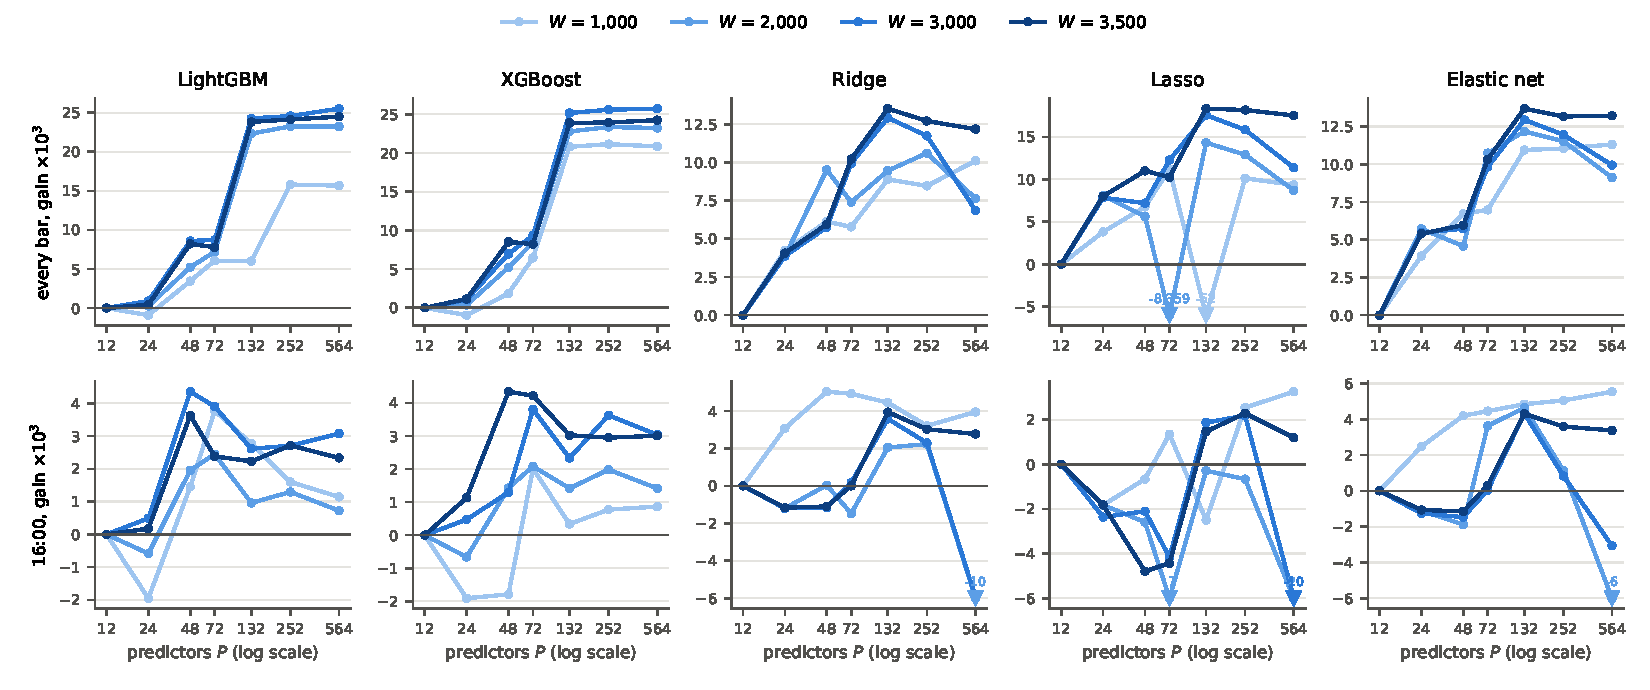
\includegraphics[width=\linewidth]{figures/rehaul_complexity_features.pdf}
  \caption{Feature scaling: the gain over the HAR benchmark set against the number of predictors $P = 12 + 12k$
    ($k = 0, 1, 3, 5, 10, 20, 46$ exogenous series), one line per rolling window ($W = \rhcxWOne$, \rhcxWTwo,
    \rhcxWMain{} and \rhcxWLong{} trading days, $T = 13W$ bars), one panel per model. Gain: QLIKE of the same
    window's $k = 0$ rung minus the rung's, $\times 10^3$, on the \rhcxNBars{} scored bars (top) and the 16:00 bar
    (bottom). Monthly refits at \rhcxNOrigins{} origins. FOMC-patched design.}
  \label{fig:rh_cx_features}
\end{figure}
\begin{figure}[tbp]
  \centering
  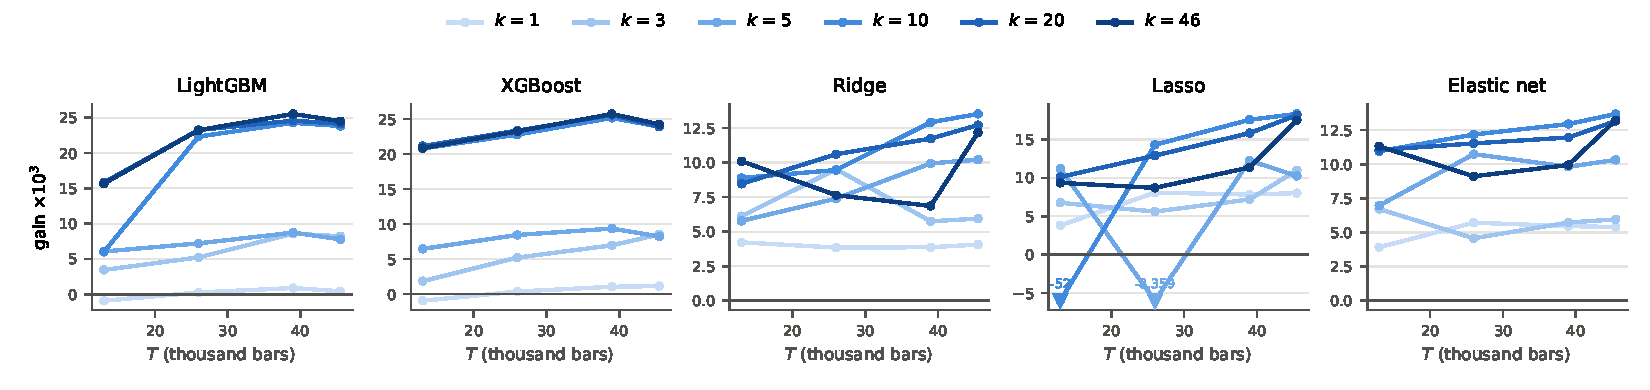
\includegraphics[width=\linewidth]{figures/rehaul_complexity_data.pdf}
  \caption{Data scaling: the gain over the same window's $k = 0$ rung against the window length $T$ at a fixed number
    of exogenous series $k$ (every bar). Same runs as Figure~\ref{fig:rh_cx_features}. FOMC-patched design.}
  \label{fig:rh_cx_data}
\end{figure}
